\newpage

\section{Theory}
\label{sec:theory}


% ----------------------------
%  Motivation
% ----------------------------
\subsection{Motivation}
\label{subsec:motivation}

The shock angle $\beta$ is a key parameter in the analysis of supersonic flows, as it determines the region of influence of disturbances and the behavior of shock waves. The shock angle is defined as the angle between the shock wave and the direction of the incoming flow. It is related to the Mach number of the flow and the angle of attack of the object causing the shock wave.
\begin{equation}
	M_{n1}=M_\infty\sin\beta
\end{equation}
\vspace{4pt}
\begin{minipage}{0.48\linewidth}
\textit{(a) Pressure behind the shock}
\[
	\frac{p_2}{p_\infty}
	\;=\;
	1+\frac{2\gamma}{\gamma+1}\Bigl(M_{n1}^2-1\Bigr),
	\qquad
\]
\end{minipage}
\hfill
\begin{minipage}{0.48\linewidth}
\textit{(b) Local pressure coefficient}
\[
	C_{p,2}
	\;=\;
	\frac{p_2-p_\infty}{\tfrac12\gamma p_\infty M_\infty^2}
	\;=\;
	\frac{2}{\gamma M_\infty^{2}}\!
	\Bigl(\tfrac{p_2}{p_\infty}-1\Bigr).
\]
\end{minipage}

So Knowing the Mach angle allows us to verify the validity of theory and the numerical method. The Mach angle is a key parameter in the analysis of supersonic flows, as it determines the region of influence of disturbances and the behavior of shock waves. 


In the \emph{small‐disturbance limit} ($\theta\ll1$, $\beta\approx\mu$) these formulas degenerate to the familiar linear results
\[
	C_p \;\approx\; \frac{2\theta}{\sqrt{M_\infty^{2}-1}},
	\qquad
	C_L \;\approx\; -\,\frac{2\theta^{2}}{\sqrt{M_\infty^{2}-1}},
	\qquad
	C_D \;\approx\; \frac{2\theta^{2}}{\sqrt{M_\infty^{2}-1}}.
\]


% ----------------------------
%  Hypothesis
% ----------------------------
\subsection{Hypothesis}
\label{subsec:hypothesis}

\begin{itemize}
\item Inviscid, adiabatic, perfect-gas flow, steady
	\begin{equation*}
		P = \rho R T \quad ; \quad \gamma = const \quad ; \quad div(v) = 0 \quad ; \quad \frac{\partial }{\partial t} = 0
	\end{equation*}

\item Small perturbations of the flow field
	\begin{equation*}
		v = v_0 + v' \quad ; \quad P = P_0 + P' \quad ; \quad T = T_0 + T'
	\end{equation*}

\item Disturbance velocities
	\begin{equation*}
		v' = \epsilon v_1 + \epsilon^2 v_2 + \epsilon^3 v_3 + ... \quad ; \quad \epsilon << 1
	\end{equation*}

\end{itemize}


% ----------------------------
%  Governing equations
% ----------------------------
\subsection{Governing equations}
\label{subsec:governing_equations}
The full compressible potential equation, which is a second-order partial differential equation, can be expressed in terms of the velocity potential $\phi$ as follows:
\begin{equation}
	(1 - M^2\phi_x^2)\phi_{xx} - 2M^2\phi_x\phi_y\phi_{xy} + (1 - M^2\phi_y^2)\phi_{yy} + \phi_{zz} = 0,
\end{equation}
\label{eq:governing_equations}
where $M$ is the Mach number, and $\phi_x$, $\phi_y$, and $\phi_z$ are the partial derivatives of the velocity potential with respect to the spatial coordinates $x$, $y$, and $z$, respectively. The subscripts denote partial differentiation.

\subsection{Linearized equations}
\label{subsec:linearized_equations}
The linearized equations are obtained by substituting the perturbation velocities into the governing equations and neglecting higher-order terms. The resulting equations can be expressed as follows:
\begin{equation}
	(1 - M_\infty^2) \phi_{xx} + \phi_{yy} + \phi_{zz} = 0.
	\label{eq:small-disturb}
\end{equation}
	
This limited development neglects all terms of order \(O(\phi_x^2)\) and above, as well as shock-shock interactions, thereby restricting valid Mach and deflection ranges.


% ----------------------------
%  Shock angle
% ----------------------------
\subsection{Shock angle}

% ----- Exact relation -----
\subsubsection{Exact relation}
The exact oblique-shock relation for a wedge half-angle \(\theta\) is given by the following equation in the \textit{NASA Technical Paper 1406}:
\begin{equation}
	tan\theta = 2\cot\beta\frac{M_\infty^2\sin^2\beta - 1}{M_\infty^2(\gamma+\cos2\beta)+2}.
\end{equation}
\label{eq:shock_angle}

This equation cannot be solved analytically for \(\beta\) in terms of \(\theta\) and \(M_\infty\).In fact it's a transcendental equation. However, we can use the bisection method to find the solution numerically. 

% ----- Numerical solution -----
\subsubsection{Numerical solution}
As mentionned above the equation \ref{eq:shock_angle} is not analytically solvable for \(\beta\). We can then use the bisection method to find the solution numerically. The bisection method is a root-finding algorithm that repeatedly bisects an interval and selects the subinterval in which a root exists. It is a simple and robust method for finding roots of continuous functions.

Therefore, you will find below the Python code that implements the bisection method to find the shock angle \(\beta\) for a given deflection angle \(\theta\) and Mach number \(M_\infty\). The code is organized into several functions, each responsible for a specific task in the process of finding the shock angle.

\begin{enumerate}[label=- , leftmargin=*, itemsep=1em]
    \item \textbf{Computation from \(\beta\) to \(\theta\):} \\
    The function \texttt{theta\_from\_beta(beta, M, gamma)} computes the deflection angle \(\theta\) from the shock angle \(\beta\) using the exact oblique-shock relation:
    \[
    \theta = \arctan\!\Biggl( \frac{2\cot\beta\, (M^2\sin^2\beta - 1)}{M^2\left(\gamma + \cos2\beta\right)+2} \Biggr).
    \]
	\begin{pycode}
def theta_from_beta(beta, M, gamma=1.4):
	"""
	Returns theta (rad) for an oblique shock.
	Accepts beta as scalar or numpy array.
	"""
	beta = np.asarray(beta)
	term1 = 2.0 / np.tan(beta)
	term2 = M**2 * np.sin(beta)**2 - 1.0
	term3 = M**2 * (gamma + np.cos(2.0 * beta)) + 2.0
	return np.arctan(term1 * term2 / term3) 
	\end{pycode}


    \item \textbf{Bisection Method:} \\
    The function \texttt{bisection(beta\_low, beta\_high, f, tol, max\_iter)} applies the bisection method to solve 
    \[
    f(\beta) = \theta(\beta) - \theta_{\text{target}} = 0,
    \]
    where \(\theta_{\text{target}}\) is the prescribed deflection angle. It refines the interval \([\beta_{\text{low}}, \beta_{\text{high}}]\) until the value of \(f(\beta)\) is within a specified tolerance.
	\begin{pycode}
def bisection(beta_low, beta_high, f, tol=1e-10, max_iter=100):
	"""Find root of f(beta)=0 using bisection method (beta in rad)."""
	f_low = f(beta_low)
	for _ in range(max_iter):
		beta_mid = 0.5 * (beta_low + beta_high)
		f_mid = f(beta_mid)
		if abs(f_mid) < tol:
			return beta_mid
		if f_low * f_mid < 0.0:
			beta_high = beta_mid
		else:
			beta_low, f_low = beta_mid, f_mid
	raise RuntimeError("Bisection_did_not_converge.")	
	\end{pycode}


	\item \textbf{Bracket Finding:} \\
	The function \texttt{bracket\_roots(theta\_rad, M, gamma, n\_scan)} scans a range of \texttt{beta} values—from the Mach angle \(\sin^{-1}(1/M)\) up to nearly \(90^\circ\)—to detect intervals where \(f(\beta)\) changes sign. These intervals are the candidate regions where a root exists.
	\begin{pycode}
def bracket_roots(theta_rad, M, gamma=GAMMA, n_scan=4000):
	"""
	Scan beta from Mach line to 89.9deg:
	returns list of intervals [beta_low, beta_high] where f changes sign.
	"""
	beta_min = math.asin(1.0 / M) + 1e-6
	beta_max = math.radians(89.9)

	betas = np.linspace(beta_min, beta_max, n_scan)
	f_vals = theta_from_beta(betas, M, gamma) - theta_rad

	idx = np.where(np.diff(np.sign(f_vals)))[0]
	return [(betas[i], betas[i + 1]) for i in idx]
	\end{pycode}


	\item \textbf{Determining \texttt{beta} Solutions:} \\
	The function \texttt{beta\_solutions(theta\_deg, M, gamma)} computes the shock angle(s) for a given deflection angle \(\theta\) (converted from degrees to radians). It uses the previously identified bracketing intervals and applies the bisection method within each interval to accurately compute the corresponding \texttt{beta} values. Depending on the case, it may return one or two solutions (typically corresponding to the weak and strong shock cases).
	\begin{pycode}
def beta_solutions(theta_deg, M, gamma=GAMMA):
	"""
	Returns a list [beta_weak (rad), beta_strong (rad) (optional)]
	for a given (theta, M) pair. 0 or 1 or 2 solutions.
	"""
	theta_rad = math.radians(theta_deg)
	intervals = bracket_roots(theta_rad, M, gamma)
	betas = []
	for beta_low, beta_high in intervals:
		betas.append(
			bisection(beta_low, beta_high,
				lambda b: theta_from_beta(b, M, gamma) 
				- theta_rad))
	return betas
	\end{pycode}
\end{enumerate}

With the code below it is possible to solve $\beta$ for arrays of \(\theta\) and \(M_\infty\) values. By doing so and plotting the results, we can compare the numerical solution with the analytical solution given by the code with a reviewed version from \cite{Tables de Détente ou de Choc by Supaero}. 
\begin{figure}[H]
    \centering
    \begin{minipage}[b]{0.45\linewidth}
        \centering
        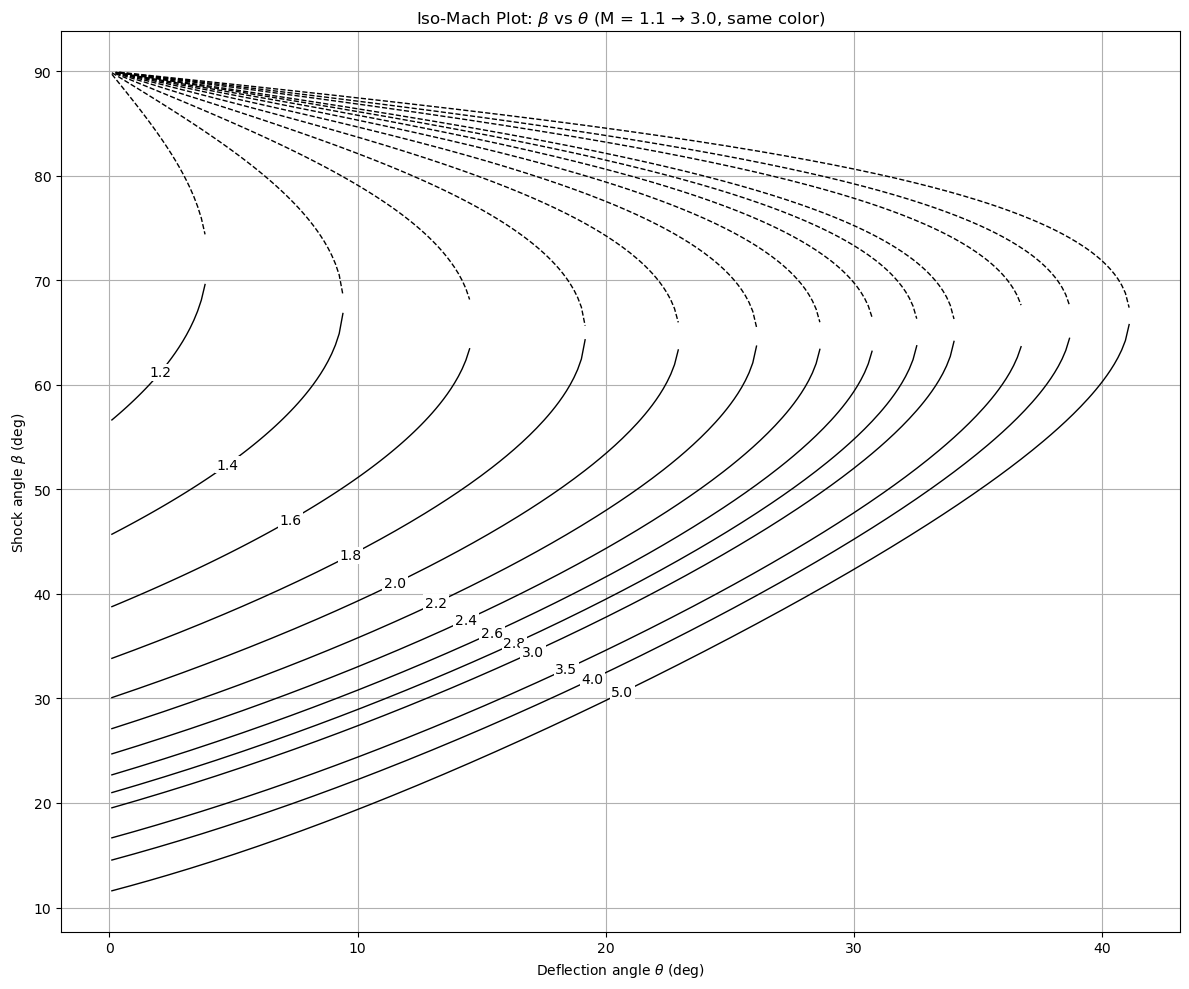
\includegraphics[width=\linewidth]{ressources/figures/compute_polaire.png}
		\caption{Computed polar}
    \end{minipage}
    \begin{minipage}[b]{0.45\linewidth}
        \centering
        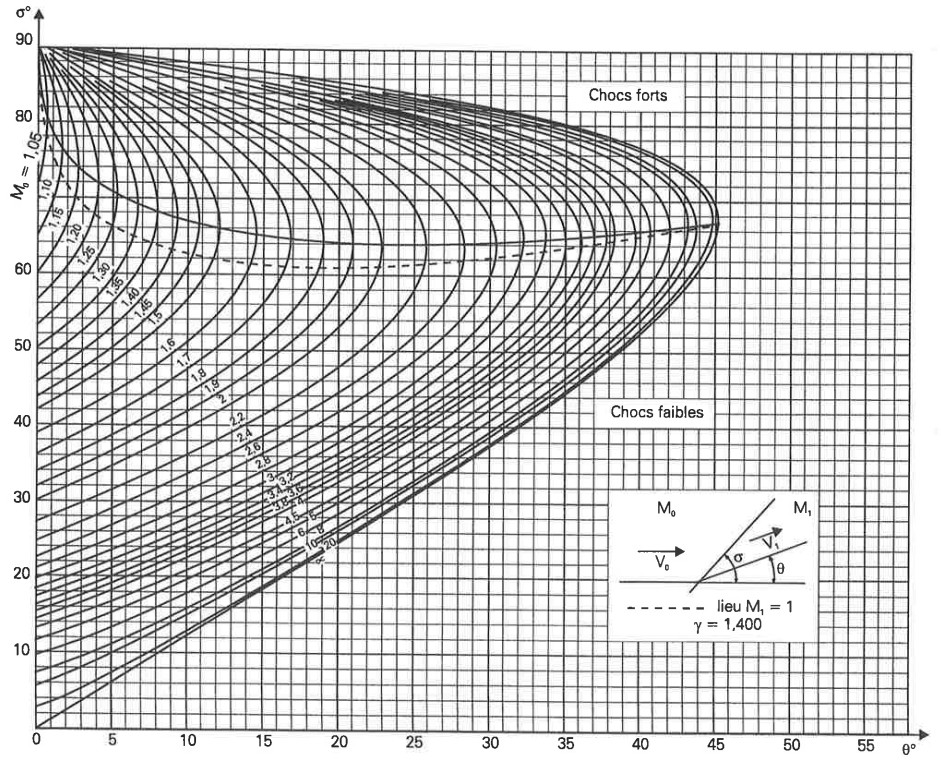
\includegraphics[width=\linewidth]{ressources/figures/supaero_polar.jpg}
		\caption{Supaero polar}
    \end{minipage}
    \label{fig:polar_comparison}
\end{figure}

We can see that the results are similar showing this resolution is valid. The difference between the two results is due to the fact that the code from Supaero is using a diffrent type of plotting.

% ----- Linearized shock angle -----
\subsubsection{Linearized shock angle}
Because the formal solution is complex to compute, we can use the small-disturbance approximation to obtain a linearized version of the shock angle. In the limit \(\theta\to0\) with attached flow, the critical condition arises when the numerator vanishes:
\begin{align}
	&M_\infty^2\sin^2\beta_d - 1 \approx 0\\
	\Longrightarrow \quad &\beta_d \approx \sin^{-1}\Bigl(\frac{1}{M_\infty}\Bigr)
\end{align}
\label{eq:beta_d}

Then the equation below offers a first-order shock-detachment estimate. Note the distinction from the Mach angle \(\mu=\sin^{-1}(1/M_\infty)\), which applies to infinitesimal disturbances rather than finite shocks.


\begin{center}
	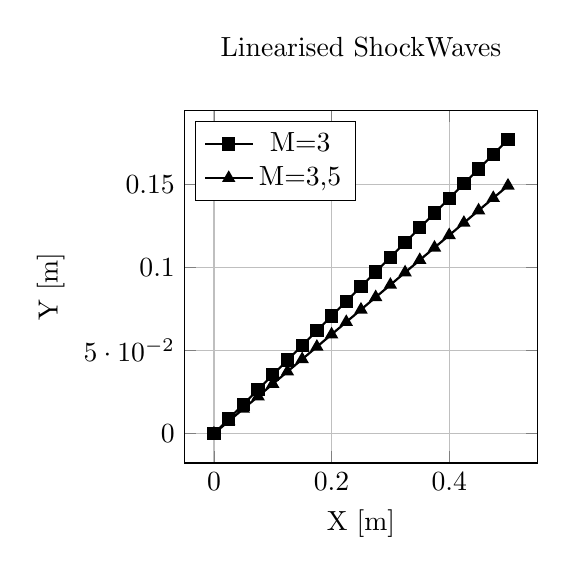
\begin{tikzpicture}
	  \begin{axis}[
		width=0.5\textwidth,
		height=0.5\textwidth,
		xlabel={X [m]},
		ylabel={Y [m]},
		title={Linearised ShockWaves},
		title style={yshift=10pt},
		grid=major,
		legend style={legend pos=north west},
		% scaled x ticks=false,  % éventuellement pour afficher en pleine valeur
	  ]
		\addplot[
		  smooth,
		  mark=square*,
		  thick,
		] coordinates {
			(0, 0)
			(0.025, 0.008838835)
			(0.05, 0.01767767)
			(0.075, 0.026516504)
			(0.1, 0.035355339)
			(0.125, 0.044194174)
			(0.15, 0.053033009)
			(0.175, 0.061871843)
			(0.2, 0.070710678)
			(0.225, 0.079549513)
			(0.25, 0.088388348)
			(0.275, 0.097227182)
			(0.3, 0.106066017)
			(0.325, 0.114904852)
			(0.35, 0.123743687)
			(0.375, 0.132582521)
			(0.4, 0.141421356)
			(0.425, 0.150260191)
			(0.45, 0.159099026)
			(0.475, 0.167937861)
			(0.5, 0.176776695)		
		};
		\addlegendentry{M=3};
	
		\addplot[
		  smooth,
		  mark=triangle*,
		  thick,
		] coordinates {
			(0, 0)
			(0.025, 0.00745356)
			(0.05, 0.01490712)
			(0.075, 0.02236068)
			(0.1, 0.02981424)
			(0.125, 0.0372678)
			(0.15, 0.04472136)
			(0.175, 0.052174919)
			(0.2, 0.059628479)
			(0.225, 0.067082039)
			(0.25, 0.074535599)
			(0.275, 0.081989159)
			(0.3, 0.089442719)
			(0.325, 0.096896279)
			(0.35, 0.104349839)
			(0.375, 0.111803399)
			(0.4, 0.119256959)
			(0.425, 0.126710519)
			(0.45, 0.134164079)
			(0.475, 0.141617639)
			(0.5, 0.149071198)
		};
		\addlegendentry{M=3,5};
	
	  \end{axis}
	\end{tikzpicture}
\end{center}
